% Heaps -- Metropolis beamer slides
% Compile: pdflatex heaps.tex (x2)
\documentclass[10pt,aspectratio=169]{beamer}

\usetheme{metropolis}
\metroset{block=fill, numbering=fraction, progressbar=frametitle}

\usepackage[T1]{fontenc}
\usepackage{amsmath, amssymb}
\usepackage{listings}
\usepackage{booktabs}
\usepackage{tikz}
\usetikzlibrary{arrows.meta, positioning, calc, trees}

% ---- colors -------------------------------------------------------------
\definecolor{mLightBlue}{HTML}{4C72B0}
\definecolor{mGreen}{HTML}{55A868}
\definecolor{mRed}{HTML}{C44E52}
\definecolor{mGray}{HTML}{BFBFBF}
\setbeamercolor{alerted text}{fg=mRed}

% ---- code style ---------------------------------------------------------
\lstdefinestyle{jl}{
  basicstyle=\ttfamily\footnotesize,
  keywordstyle=\color{mRed}\bfseries,
  commentstyle=\color{mGreen}\itshape,
  numberstyle=\tiny\color{mGray},
  showstringspaces=false,
  breaklines=true,
  columns=fullflexible,
  morekeywords={function,for,in,if,else,elseif,end,return,length,while,push,pop,div,error,isempty}
}
\lstset{style=jl}

% ---- tree node styles ---------------------------------------------------
\tikzset{
  hnode/.style={draw, circle, minimum size=8mm, inner sep=0pt, font=\small, fill=mLightBlue!20},
  hswap/.style={hnode, fill=mRed!25},
}

% ---- shared tree command ------------------------------------------------
\newcommand{\heaptree}[1]{%
  \begin{tikzpicture}[scale=1.0,
    level distance=1.2cm,
    level 1/.style={sibling distance=3.6cm},
    level 2/.style={sibling distance=1.8cm},
    level 3/.style={sibling distance=0.9cm},
    every node/.style={hnode}]
    #1
  \end{tikzpicture}%
}

% ---- title --------------------------------------------------------------
\title{Heaps}
\subtitle{Data Structures \& Algorithms}
\date{}
\author{}

\begin{document}

\maketitle

% =========================================================================
\section{The Heap Property}

\begin{frame}{What is a Heap?}
  A \alert{heap} is a nearly complete binary tree satisfying the \alert{heap property}.

  \bigskip
  \begin{columns}[c]
    \begin{column}{0.52\textwidth}
      \begin{block}{Min-Heap Property}
        For every node $i$ other than the root:
        \[
          A[\mathrm{parent}(i)] \le A[i].
        \]
        The \alert{smallest} element is at the root.
      \end{block}

      \bigskip
      We focus on \alert{min-heaps} throughout.\\
      Max-heaps are symmetric (flip $\le$ to $\ge$).
    \end{column}
    \begin{column}{0.42\textwidth}
      \begin{center}
      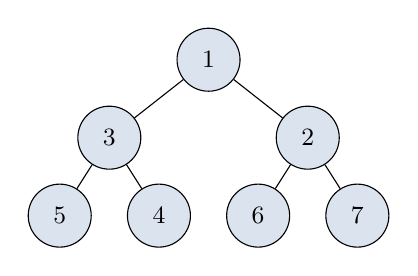
\begin{tikzpicture}[scale=0.9,
        level distance=1.1cm,
        level 1/.style={sibling distance=2.8cm},
        level 2/.style={sibling distance=1.4cm},
        every node/.style={hnode}]
        \node {1}
          child { node {3}
            child { node {5} }
            child { node {4} }
          }
          child { node {2}
            child { node {6} }
            child { node {7} }
          };
      \end{tikzpicture}
      \end{center}
    \end{column}
  \end{columns}
\end{frame}

% =========================================================================
\section{Array Representation}

\begin{frame}{Storing a Heap in an Array}
  A heap on $n$ elements is stored in an array $A[1:n]$.
  The tree structure is \alert{implicit}:
  \[
    \mathrm{parent}(i) = \lfloor i/2 \rfloor, \qquad
    \mathrm{left}(i)   = 2i, \qquad
    \mathrm{right}(i)  = 2i+1.
  \]

  \pause
  \bigskip
  \begin{center}
  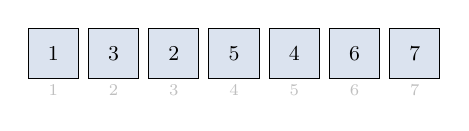
\begin{tikzpicture}[scale=0.85, every node/.style={transform shape}]
    \foreach \v [count=\i from 1] in {1,3,2,5,4,6,7} {
      \node[draw, minimum size=7.5mm, fill=mLightBlue!20, font=\small]
        at (\i*0.9-0.45, 0) {\v};
      \node[font=\scriptsize, mGray] at (\i*0.9-0.45, -0.55) {\i};
    }
  \end{tikzpicture}
  \end{center}

  \bigskip
  \begin{center}
    \alert{Leaves} are at positions $\lfloor n/2 \rfloor + 1, \ldots, n$
    (no child index fits in the array).
  \end{center}
\end{frame}

\begin{frame}{The Tree Behind the Array}
  $A = [1,\ 3,\ 2,\ 5,\ 4,\ 6,\ 7]$

  \bigskip
  \begin{center}
  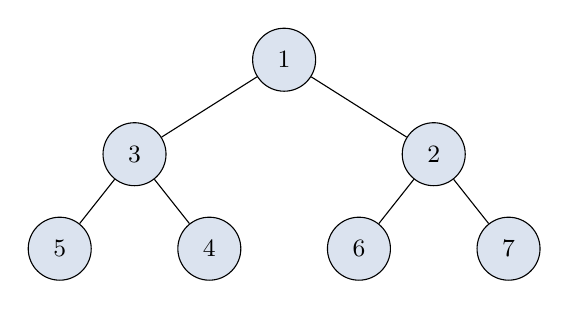
\begin{tikzpicture}[scale=1.0,
    level distance=1.2cm,
    level 1/.style={sibling distance=3.8cm},
    level 2/.style={sibling distance=1.9cm},
    every node/.style={hnode}]
    \node {1}
      child { node {3}
        child { node {5} }
        child { node {4} }
      }
      child { node {2}
        child { node {6} }
        child { node {7} }
      };
  \end{tikzpicture}
  \end{center}

  \bigskip
  \begin{center}
    Every parent is $\le$ its children. $\quad$ Root = minimum.
  \end{center}
\end{frame}

% =========================================================================
\section{Heapify}

\begin{frame}{The Core Subroutine: \texttt{heapify}}
  \textbf{Assumption}: the subtrees rooted at \texttt{left(i)} and
  \texttt{right(i)} are valid min-heaps.

  \bigskip
  \textbf{Goal}: fix a possible violation at node $i$ by \alert{floating
  $A[i]$ downward}.

  \bigskip
  \begin{enumerate}
    \item Find the smallest among $A[i]$, $A[\mathrm{left}(i)]$, $A[\mathrm{right}(i)]$.
    \item If $A[i]$ is not the smallest, swap it with the smallest child.
    \item Recurse on the subtree where the swap landed.
  \end{enumerate}
\end{frame}

\begin{frame}{\texttt{heapify} in Action}
  Call \texttt{heapify!(A, 1)} after $A[1]$ was changed to $9$.
  Violation: $9 > 3$ and $9 > 2$.

  \bigskip
  \begin{center}
  \heaptree{
    \node[hswap] {9}
      child { node[hswap] {2}
        child { node {5} }
        child { node {4} }
      }
      child { node {3}
        child { node {6} }
        child { node {7} }
      };
  }
  \end{center}
\end{frame}

\begin{frame}{\texttt{heapify} in Action}
  Smallest child is $2$: swap $9 \leftrightarrow 2$.
  Recurse: $9 > 5$ and $9 > 4$, violation at new position.

  \bigskip
  \begin{center}
  \heaptree{
    \node {2}
      child { node[hswap] {9}
        child { node[hswap] {4}
        }
        child { node {5} }
      }
      child { node {3}
        child { node {6} }
        child { node {7} }
      };
  }
  \end{center}
\end{frame}

\begin{frame}{\texttt{heapify} in Action}
  Smallest child is $4$: swap $9 \leftrightarrow 4$.
  Now $9$ is a leaf — heap property restored.

  \bigskip
  \begin{center}
  \heaptree{
    \node {2}
      child { node {4}
        child { node {9} }
        child { node {5} }
      }
      child { node {3}
        child { node {6} }
        child { node {7} }
      };
  }
  \end{center}
\end{frame}

\begin{frame}[fragile]{\texttt{heapify}: Code}
\begin{lstlisting}
function heapify!(A, i)
    n = length(A)
    l = 2i;   r = 2i + 1
    smallest = i

    if l <= n && A[l] < A[smallest]
        smallest = l
    end
    if r <= n && A[r] < A[smallest]
        smallest = r
    end

    if smallest != i
        A[i], A[smallest] = A[smallest], A[i]   # swap down
        heapify!(A, smallest)                    # recurse
    end
end
\end{lstlisting}

  \bigskip
  \textbf{Running time}: height $h = \lfloor \log_2 n \rfloor$,
  each level $O(1)$ work $\Rightarrow$ $O(\log n)$.
\end{frame}

% =========================================================================
\section{Building a Heap}

\begin{frame}[fragile]{Building a Heap from Scratch}
  Call \texttt{heapify} bottom-up on every \alert{internal} node
  (leaves already satisfy the property).

\begin{lstlisting}
function build_heap!(A)
    for i in div(length(A), 2):-1:1
        heapify!(A, i)
    end
end
\end{lstlisting}

  \bigskip
  \begin{center}
    Start at $\lfloor n/2 \rfloor$ and work down to $1$.
  \end{center}
\end{frame}

\begin{frame}{Why \texttt{build\_heap} is $O(n)$}
  Naively: $O(n/2)$ calls each costing $O(\log n)$ $\Rightarrow$ $O(n \log n)$.

  \bigskip
  But nodes near the leaves do \alert{little work}.
  There are $\approx n/2^{h+1}$ nodes at height $h$, and \texttt{heapify}
  at height $h$ costs $O(h)$:
  \[
    \sum_{h=0}^{\lfloor \log n \rfloor}
    \left\lceil \frac{n}{2^{h+1}} \right\rceil O(h)
    = O\!\left(n \sum_{h=0}^{\infty} \frac{h}{2^h}\right) = O(n),
  \]
  using $\displaystyle\sum_{h=0}^{\infty} h\,x^h = \dfrac{x}{(1-x)^2}$ with $x = \tfrac{1}{2}$.
\end{frame}

% =========================================================================
\section{Heap Operations}

\begin{frame}{Extract-Min}
  Remove and return the root (the minimum).

  \begin{enumerate}
    \item Save \texttt{A[1]}.
    \item Move the \alert{last} element to the root; shrink the array.
    \item Call \texttt{heapify!(A, 1)} to restore the heap.
  \end{enumerate}
\end{frame}

\begin{frame}{Extract-Min in Action}
  Starting heap $A = [1,3,2,5,4,6,7]$.
  Extract $\min = 1$; move last element $7$ to the root.

  \bigskip
  \begin{columns}[c]
    \begin{column}{0.45\textwidth}
      \begin{center}
        \textbf{Before}\\[4pt]
        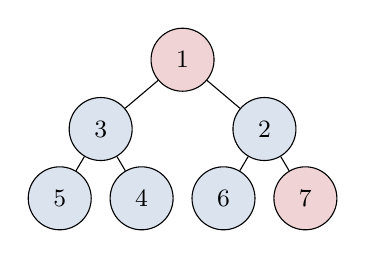
\begin{tikzpicture}[scale=0.8,
          level distance=1.1cm,
          level 1/.style={sibling distance=2.6cm},
          level 2/.style={sibling distance=1.3cm},
          every node/.style={hnode}]
          \node[hswap] {1}
            child { node {3}
              child { node {5} }
              child { node {4} }
            }
            child { node {2}
              child { node {6} }
              child { node[hswap] {7} }
            };
        \end{tikzpicture}
      \end{center}
    \end{column}
    \begin{column}{0.45\textwidth}
      \begin{center}
        \textbf{After moving 7 to root}\\[4pt]
        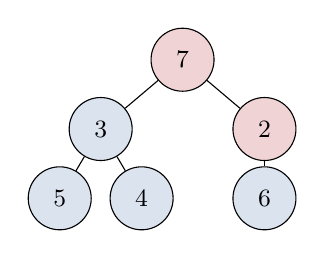
\begin{tikzpicture}[scale=0.8,
          level distance=1.1cm,
          level 1/.style={sibling distance=2.6cm},
          level 2/.style={sibling distance=1.3cm},
          every node/.style={hnode}]
          \node[hswap] {7}
            child { node {3}
              child { node {5} }
              child { node {4} }
            }
            child { node[hswap] {2}
              child { node {6} }
            };
        \end{tikzpicture}
      \end{center}
    \end{column}
  \end{columns}

  \bigskip
  \begin{center}
    Heap size reduced to 6. Now call \texttt{heapify!(A, 1)}.
  \end{center}
\end{frame}

\begin{frame}{Extract-Min in Action}
  Heapify at root: smallest child of $7$ is $\min(3,2)=2$. Swap $7 \leftrightarrow 2$.

  \bigskip
  \begin{columns}[c]
    \begin{column}{0.45\textwidth}
      \begin{center}
        \textbf{After swap $7 \leftrightarrow 2$}\\[4pt]
        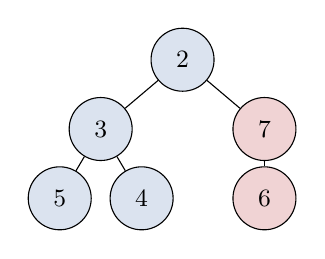
\begin{tikzpicture}[scale=0.8,
          level distance=1.1cm,
          level 1/.style={sibling distance=2.6cm},
          level 2/.style={sibling distance=1.3cm},
          every node/.style={hnode}]
          \node {2}
            child { node {3}
              child { node {5} }
              child { node {4} }
            }
            child { node[hswap] {7}
              child { node[hswap] {6} }
            };
        \end{tikzpicture}
      \end{center}
    \end{column}
    \begin{column}{0.45\textwidth}
      \begin{center}
        \textbf{After swap $7 \leftrightarrow 6$, done}\\[4pt]
        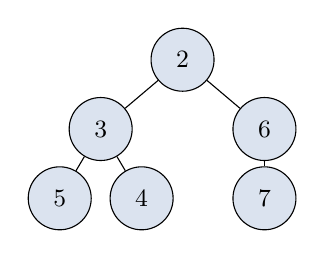
\begin{tikzpicture}[scale=0.8,
          level distance=1.1cm,
          level 1/.style={sibling distance=2.6cm},
          level 2/.style={sibling distance=1.3cm},
          every node/.style={hnode}]
          \node {2}
            child { node {3}
              child { node {5} }
              child { node {4} }
            }
            child { node {6}
              child { node {7} }
            };
        \end{tikzpicture}
      \end{center}
    \end{column}
  \end{columns}

  \bigskip
  \begin{center}
    $7$ is a leaf — heap property restored. \quad Result: $A = [2,3,6,5,4,7]$.
  \end{center}
\end{frame}

\begin{frame}[fragile]{Extract-Min: Code}
\begin{lstlisting}
function heap_extract_min!(A)
    min_val = A[1]
    A[1] = A[end]
    pop!(A)
    heapify!(A, 1)
    return min_val
end
\end{lstlisting}

  \textbf{Running time}: $O(\log n)$.
\end{frame}

\begin{frame}{Decrease-Key}
  Lower $A[i]$ to \texttt{key} and \alert{bubble up} to restore the heap.

  \begin{enumerate}
    \item If \texttt{key} $>$ \texttt{A[i]}: error (can only decrease).
    \item Set \texttt{A[i] = key}.
    \item While \texttt{A[i]} $<$ its parent: swap upward.
  \end{enumerate}
\end{frame}

\begin{frame}{Decrease-Key in Action}
  Heap $A = [2,3,6,5,4,7]$. Decrease $A[6] = 7$ to $1$.

  \bigskip
  \begin{columns}[c]
    \begin{column}{0.30\textwidth}
      \begin{center}
        \textbf{Original}\\[4pt]
        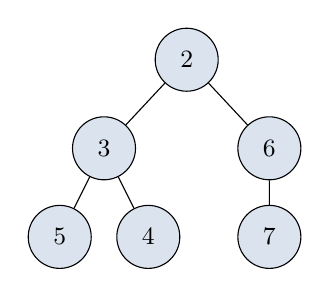
\begin{tikzpicture}[scale=0.75,
          level distance=1.5cm,
          level 1/.style={sibling distance=2.8cm},
          level 2/.style={sibling distance=1.5cm},
          every node/.style={hnode}]
          \node {2}
            child { node {3}
              child { node {5} }
              child { node {4} }
            }
            child { node {6}
              child { node {7} }
            };
        \end{tikzpicture}
      \end{center}
    \end{column}
    \begin{column}{0.30\textwidth}
      \begin{center}
        \textbf{$A[6] \leftarrow 1$ (violation)}\\[4pt]
        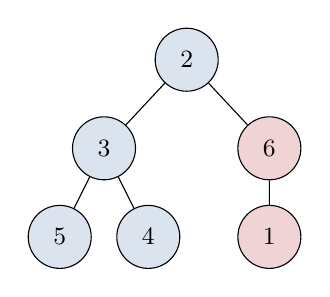
\begin{tikzpicture}[scale=0.75,
          level distance=1.5cm,
          level 1/.style={sibling distance=2.8cm},
          level 2/.style={sibling distance=1.5cm},
          every node/.style={hnode}]
          \node {2}
            child { node {3}
              child { node {5} }
              child { node {4} }
            }
            child { node[hswap] {6}
              child { node[hswap] {1} }
            };
        \end{tikzpicture}
      \end{center}
    \end{column}
    \begin{column}{0.30\textwidth}
      \begin{center}
        \textbf{Swap $1 \leftrightarrow 6$}\\[4pt]
        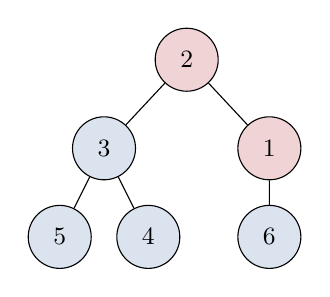
\begin{tikzpicture}[scale=0.75,
          level distance=1.5cm,
          level 1/.style={sibling distance=2.8cm},
          level 2/.style={sibling distance=1.5cm},
          every node/.style={hnode}]
          \node[hswap] {2}
            child { node {3}
              child { node {5} }
              child { node {4} }
            }
            child { node[hswap] {1}
              child { node {6} }
            };
        \end{tikzpicture}
      \end{center}
    \end{column}
  \end{columns}

  \bigskip
  \begin{center}
    $1 < 6$: swap. Then $1 < 2$: swap again.
  \end{center}
\end{frame}

\begin{frame}{Decrease-Key in Action}
  After swap $1 \leftrightarrow 2$: $1$ reaches the root. Heap property restored.

  \bigskip
  \begin{center}
    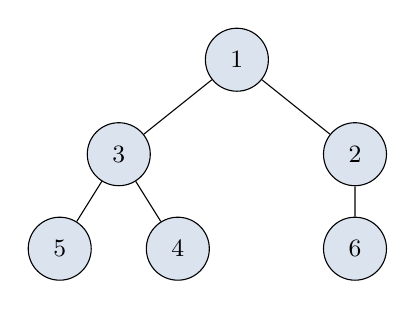
\begin{tikzpicture}[scale=1.0,
      level distance=1.2cm,
      level 1/.style={sibling distance=3.0cm},
      level 2/.style={sibling distance=1.5cm},
      every node/.style={hnode}]
      \node {1}
        child { node {3}
          child { node {5} }
          child { node {4} }
        }
        child { node {2}
          child { node {6} }
        };
    \end{tikzpicture}
  \end{center}

  \bigskip
  \begin{center}
    Result: $A = [1,3,2,5,4,6]$.
    The decreased key bubbled up 2 levels.
  \end{center}
\end{frame}

\begin{frame}[fragile]{Decrease-Key: Code}
\begin{lstlisting}
function heap_decrease_key!(A, i, key)
    key > A[i] && error("new key is larger than current key")
    A[i] = key
    while i > 1 && A[div(i, 2)] > A[i]
        A[i], A[div(i, 2)] = A[div(i, 2)], A[i]
        i = div(i, 2)
    end
end
\end{lstlisting}

  \textbf{Running time}: node travels at most $O(\log n)$ levels upward $\Rightarrow$ $O(\log n)$.
\end{frame}

\begin{frame}[fragile]{Insert}
  Append $+\infty$ as a sentinel, then decrease it to \texttt{key}.

\begin{lstlisting}
function min_heap_insert!(A, key)
    push!(A, Inf)
    heap_decrease_key!(A, length(A), key)
end
\end{lstlisting}

  \bigskip
  \textbf{Running time}: $O(\log n)$.

  \bigskip
  \begin{center}
  \begin{tabular}{lc}
    \toprule
    Operation & Time \\
    \midrule
    \texttt{build\_heap} & $O(n)$ \\
    \texttt{extract\_min} & $O(\log n)$ \\
    \texttt{decrease\_key} & $O(\log n)$ \\
    \texttt{insert} & $O(\log n)$ \\
    \bottomrule
  \end{tabular}
  \end{center}
\end{frame}

% =========================================================================
\section{Heapsort}

\begin{frame}[fragile]{Heapsort}
  Build a min-heap, then repeatedly extract the minimum.

\begin{lstlisting}
function heapsort(A)
    build_heap!(A)
    sorted = []
    while !isempty(A)
        push!(sorted, heap_extract_min!(A))
    end
    return sorted    # sorted in increasing order
end
\end{lstlisting}
\end{frame}

\begin{frame}{Heapsort Running Time}
  \begin{itemize}
    \item \texttt{build\_heap}: $O(n)$.
    \item $n$ calls to \texttt{heap\_extract\_min}, each $O(\log n)$: total $O(n \log n)$.
  \end{itemize}

  \bigskip
  \begin{alertblock}{Total: $O(n \log n)$}
    In-place with $O(1)$ extra space (when implemented directly in the array).
  \end{alertblock}

  \bigskip
  \begin{center}
    \textbf{Exercise}: Trace heapsort on $[3, 1, 4, 1, 5, 9, 2, 6]$.\\
    Write the heap after each call to \texttt{heap\_extract\_min!}.
  \end{center}
\end{frame}

% =========================================================================
\section{Priority Queues}

\begin{frame}{Priority Queue}
  A \alert{priority queue} is an abstract data type supporting:
  \begin{itemize}
    \item \texttt{insert(key)} — add a new element.
    \item \texttt{extract\_min()} — remove and return the element with lowest priority.
    \item \texttt{decrease\_key(i, key)} — lower a priority.
  \end{itemize}

  \bigskip
  A min-heap implements all of these in $O(\log n)$.

  \bigskip
  \begin{block}{Classic Application: Dijkstra's Algorithm}
    A \alert{min-heap} stores vertices ordered by tentative distance.
    Each step extracts the closest unvisited vertex in $O(\log n)$
    and updates neighbours in $O(\log n)$.
  \end{block}
\end{frame}


\end{document}
